\chapter{Evaluación}
Este capítulo está dedicado a la evaluación de los resultados obtenidos por cada uno de los clasificadores. Consta de dos secciones, una dedicada a mostrar los resultados obtenidos con tablas y gráficas, y otra dedicada a la discusión de los resultados obtenidos, donde se da una perspectiva propia sobre las limitaciones y resultados obtenidos.


\section{Resultados}

    \subsection{Estimación del tamaño de ventana}
    Con respecto a los resultados de la estimación del tamaño de ventana de cada archivo se aconseja visitar el Anexo para ver un ejemplo de dos archivos EMG con sus respectivas ventanas. (Ver \ref{anexo ventana}).

    \subsection{Extracción de características}
    Todas las gráficas asociadas a cada una de las características pueden ser consultadas en el Anexo. (Ver \ref{anexo caracteristicas}).

    \subsection{Procesamiento de datos: diferentes modelos de estudio}
   	Esta sección va dedicada a mostrar cada uno de los archivos de \newline entrenamiento-testeo utilizados para el estudio. Hay que recordar que de cada uno de ellos, se sacarán 3 con el RFE, cada uno con un número diferente de características. Pueden ser consultados en el Anexo. (Ver \ref{anexo modelos}).
	
	\subsection{Selección de características: RFE}
	Para ver que características de todas las desarrolladas fueron elegidas en cada canal se aconseja visitar el Anexo. (Ver \ref{anexo rfe}).
	
    \subsection{Clasificación binaria de señales y validación cruzada}
    Esta sección está dedicada a mostrar el rendimiento de los diferentes clasificadores en los diferentes canales estudiados. Para ello se ha hecho uso de una tabla y una gráfica, obtenidas durante la ejecución del código fuente dedicado a los clasificadores. La tabla muestra los valores en bruto de la precisión media de cada clasificador, junto con su desviación típica entre paréntesis. Finalmente se muestra la gráfica asociada a dicha tabla.
    
    \begin{table}[!ht]
    \centering
    \caption{Precisión y desviación media de los clasificadores en cada canal }
    
    \vspace{0.5cm}
    \scalebox{0.68}{
            \begin{tabular}{lllll}
                \toprule
                          &     &       N = 1 &       N = 2 &       N = 5 \\
                \midrule
                \multirow{\textbf{canal 1}} & \textbf{SVM} &  0.829167 (0.0482327)	&  0.829167 (0.0482327) &    0.8375 (0.0306186) \\
                                            & \textbf{TREE}&  0.754167 (0.0980717)		&  0.729167 (0.108653) &  0.729167 (0.132419)\\
                                            & \textbf{KNN} &     0.825 (0.0520416)      &  0.829167 (0.0482327) &  0.833333 (0.0709558) \\
                \cline{1-5}
                \multirow{\textbf{canal 2}} & \textbf{SVM} &  0.733333 (0.083749) &  0.745833 (0.108173)  &    0.7375 (0.107529)  \\
                                            & \textbf{TREE} &  0.783333 (0.111492) &  0.770833 (0.101208)  &  0.766667 (0.119606)  \\
                                            & \textbf{KNN} &  0.845833 (0.0386401)  &  0.833333 (0.0372678)  &  0.841667 (0.0448764)  \\
                \cline{1-5}
                \multirow{\textbf{canal 3}} & \textbf{SVM} &    0.8375 (0.0306186)  &  0.833333 (0.0372678)  &  0.766667 (0.0980717)  \\
                                            & \textbf{TREE} &  0.758333 (0.0991281)  &    0.6875 (0.0853913)  &  0.795833 (0.0953794)  \\
                                            & \textbf{KNN} &     0.825 (0.0408248)  &  0.820833 (0.0386401)  &  0.820833 (0.0752311)  \\
                \cline{1-5}
                \multirow{\textbf{canal 4}} & \textbf{SVM} &  0.795833 (0.125968)  &  0.791667 (0.130437)  &  0.829167 (0.0276385)  \\
                                            & \textbf{TREE} &  0.708333 (0.0903312)  &  0.733333 (0.0953794)  &       0.7 (0.129502 )  \\
                                            & \textbf{KNN} &  0.833333 (0.0372678)  &  0.841667 (0.0311805)  &    0.8125 (0.0603807)  \\
                \cline{1-5}
                \multirow{\textbf{canal total}} & \textbf{SVM} &  0.819792 (0.0660124)  &  0.823958 (0.0661602)  &  0.827083 (0.0304409)  \\
                                                & \textbf{TREE} &    0.7375 (0.0593476)  &  0.740625 (0.0721237)  &  0.751042 (0.053966)  \\
                                                & \textbf{KNN} &  0.841667 (0.0169891)  &  0.845833 (0.0295731)  &  0.835417 (0.0364732)  \\
                \cline{1-5}
                \multirow{\textbf{canal 1,2}}   & \textbf{SVM} &    0.8375 (0.0125)  &   0.81875 (0.05)  &     0.775 (0.128695)  \\
                                                & \textbf{TREE} &  0.733333 (0.052125)  &  0.733333 (0.0557462)  &  0.747917 (0.077784) \\
                                                & \textbf{KNN} &  0.822917 (0.0186339)  &  0.822917 (0.0186339)  &  0.833333 (0.0315953)  \\
                \cline{1-5}
                \multirow{\textbf{canal 3,4}}   & \textbf{SVM} &    0.8375 (0.0125)  &    0.8375 (0.0125)  &    0.8375 (0.0125)  \\
                                                & \textbf{TREE} &   0.73125 (0.0682749)  &  0.735417 (0.052125)  &  0.735417 (0.0764331)  \\
                                                & \textbf{KNN} &  0.827083 (0.01932)  &     0.825 (0.0222439)  &  0.827083 (0.0320048)  \\
                \bottomrule
            \end{tabular}   
    }
    
    \end{table}
    
    



\begin{figure}
    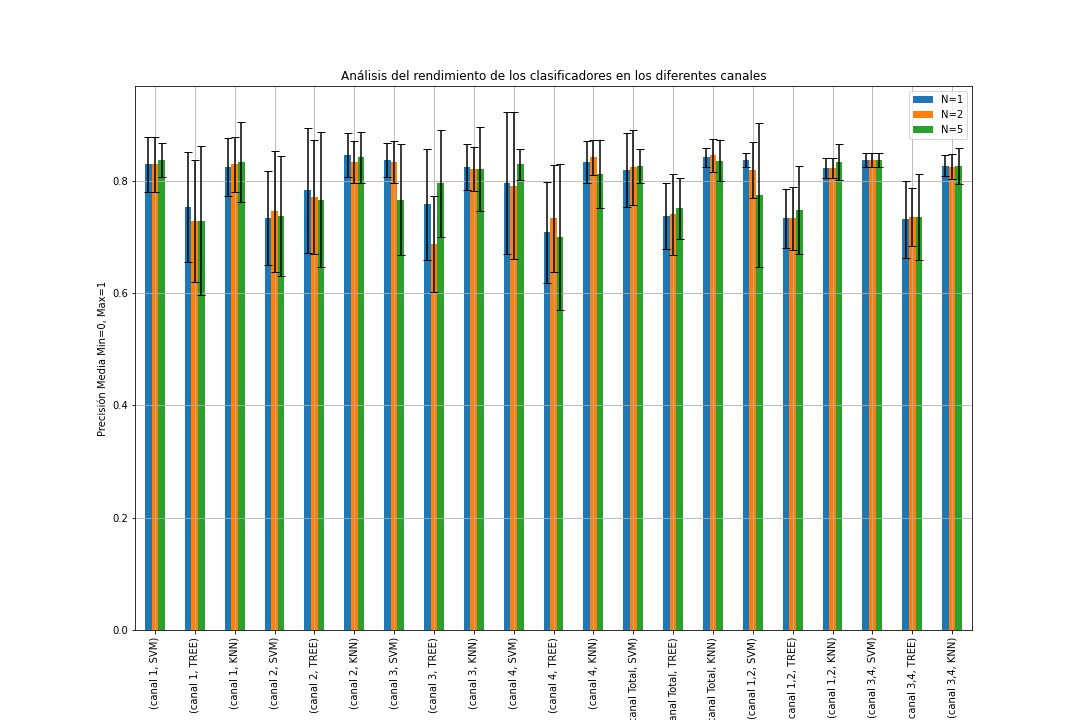
\includegraphics[width=1.0\textwidth]{imagenes/Grafica analisis final.jpg}
    \caption{Diagrama resumen de la precisión y desviación de cada clasificador}
    \label{fig:tabla resuemn}
\end{figure}

\newpage
Una vez vistas ambas tablas y la gráfica resumen de las precisiones podemos llegar a indagar en que clasificador es el más conveniente para nuestro problema. A continuación se muestra un breve resumen sobre los resultados obtenidos.
\subsubsection{Canal 1: vasto medial izquierdo}
La precisión más alta en este canal nos la da el SVM usando un archivo de entrenamiento-testeo con 5 características. 

\subsubsection{ Canal 2: recto femoral izquierdo}
En este canal la mejor precisión se obtiene con un KNN utilizando un número de vecinos de 6 y un archivo de entrenamiento-testeo con 1 característica. Su desviación típica es de las menores.

\subsubsection{Canal 3: vasto medial derecho}
En este canal la mejor precisión viene dada por un SVM con un archivo de entrenamiento-testeo con solo 1 característica. Además su desviación típica es bastante pequeña.

\subsubsection{Canal 4: recto femoral derecho}
En el canal 4 la mejor precisión nos la da un KNN utilizando un número de vecinos de 6 y un archivo de entrenamiento-testeo con 2 características.

\subsubsection{Canal 1,2: extremidad inferior izquierda}
Para el canal 1,2 el clasificador que nos da la mejor precisión es un SVM utilizando un archivo de entrenamiento-testeo con 1 característica.

\subsubsection{Canal 3,4: extremidad inferior derecha}
Para el canal 3,4 el clasificador que nos da la mejor precisión es un SVM utilizando tanto un archivo de entrenamiento-testeo con 1, 2 ó 5 características.

\subsubsection{Canal total: agrupación de todos los canales }
Para el canal total la mejor precisión viene dada por un KNN utilizando un número de vecinos de 6 y un archivo de entrenamiento-testeo con 2 características.




%4.2 Discusión
%Tras la presentación objetiva de los resultados, deberás aportar una discusión de los
%En este capítulo puedes discutir la relevancia de los resultados, presentar
%explicaciones para los resultados obtenidos (esperados o anómalos) y resaltar
%resultados que sean particularmente relevantes. Fíjate que a diferencia de la
%"Resultados", aquí se espera que incluyas tu opinión/reflexión sobre los resultados


\section{Discusión}
Como se ha ido explicando a lo largo del proyecto, la idea era desarrollar un clasificador para estimar la fatiga durante los entrenamientos y poder obtener conclusiones de anomalías en las rodillas de los pacientes y atletas. Además de esto, como ya se explicó en el capitulo \ref{tiposClasificadores}, se pretendía analizar diferentes situaciones debido a la ventaja de que la herramienta utilizada para tomar los datos llegaba a registrar los datos de 4 músculos diferentes. Por ello se optó por aumentar el estudio a diferentes niveles musculares.



\subsection{Modelos utilizados}
Los diferentes modelos que fueron utilizados para el proyecto han sido:
\begin{itemize}
\item Support vector machines (SVMs): máquinas de vector de soporte.
\item Decision trees (Trees): árboles de decisión.
\item K nearest neighbors (KNN): K vecinos más cercanos.
\end{itemize}

Viendo los resultados obtenidos (precisión y desviación) mediante la validación cruzada por cada uno de ellos, considero que el que mejor prestaciones ha dado ha sido el KNN con k = 6. Como se puede ver en la gráfica \ref{fig:tabla resuemn}, el clasificador KNN ha sido el que más estable se ha mantenido, dando en todas las situaciones estudiadas un rendimiento muy bueno y sin gran variación.

El hecho de que KNN obtenga una precisión mucho mayor a la de los árboles de decisión, pienso que se debe a que la fatiga muscular estudiada puede tener diferentes situaciones. Por ejemplo, que la fatiga esté representada en tres grupos diferentes. Estos tres grupos supongamos que tienen dichos valores:
\begin{itemize}
\item Grupo 1: RMS con valores altos, IEMG con valores bajos.
\item Grupo 2: RMS con valores bajos pero con un MNF con valores muy altos (cerca del 1).
\item Grupo 3: MAV con valores bajos y ZC con valores muy bajos (cerca del 0).
\end{itemize}

Esta situación daría 3 subgrupos representativos de la fatiga, por ello pienso que como el KNN divide todo el conjunto de datos en subgrupos, en este caso de k = 6 para determinar la nueva categoría, tiene mayor capacidad a la hora de determinar una categoría para una señal no conocida.


En segunda posición dejaría al SVM. Este clasificador también ha obtenido un buen rendimiento, pero en ciertas ocasiones una precisión muy baja y una gran variación indicada por los valores de su desviación, por lo que esto nos indica que hay veces en donde ha dado un rendimiento muy alto y otras ocasiones donde el rendimiento fue bajo. Se puede deber a que en ocasiones la fatiga no estaba realmente clara y su separación entre los vectores de soporte era muy pequeña y debido a esto el clasificador no era capaz de clasificar algunos datos correctamente.

En tercera y última posición situaría al Desion Tree. Pienso que ha sido el que peores resultados ha obtenido. En todas las situaciones estudiadas ha dado la precisión mas baja y con una gran variación.

Los árboles de decisión van realizando ramificaciones para determinar la categoría final de los datos de testeo y esto puede hacer que como no hay un patrón realmente claro en la fatiga con las características utilizadas, que no se obtenga un rendimiento del todo estable. Otra posibilidad de este rendimiento, se debe a que el conjunto de datos utilizados consta de un número mucho mayor de no fatiga = 0, que de fatiga = 1. Por ello, el árbol de decisión puede sesgar los datos al haber una clase dominante.

En conclusión, yo personalmente me quedaría con un clasificador SVM o KNN. A continuación se hace una valoración del rendimiento de cada uno de estos en los diferentes canales estudiados.

\subsection{Canal 1, canal 2, canal 3, canal 4}
Los datos obtenidos son bastantes curiosos. Podemos ver que para tanto el canal 1 como para el canal 3 (ambos registraban información del vasto medial, solo que uno de la pierna derecha y otro de la pierna izquierda) la mejor opción es el SVM.

Sin embargo, tanto para el canal 2 como para el canal 4 (ambos registraban información del recto femoral , uno en la pierna derecha y otro en la izquierda) la mejor opción es un KNN. 


Esto podría justificarse, ya que la sentadilla es un ejercicio muy demandante de vasto medial. Como se puede ver en este estudio \cite{muyor2020actividad}, donde se analiza que músculos del cuadriceps realizan una mayor activación a la hora de realizar diferentes sentadillas. Es decir, aunque el recto femoral también forma parte del cuadricpes y apoya el movimiento de la rodilla junto con el vasto medial, es el vasto medial el músculo más implicado.

Debido a esto, la señal de los canales del vasto medial puede llegar a ser más intensa que la de los canales del recto femoral. Esto puede hacer que la fatiga quede mejor definida en estos casos, ya que al tener una mayor activación, es lógico que dicho músculo se fatigue antes. Por ello pienso que los dos grupos definidos en el SVM pueden quedar definidos con una mayor separación entre los dos vectores de soporte de cada grupo y por ello clasificar mejor los datos no conocidos.

Otro factor a tener en cuenta es que la desviación típica del clasificador SVM en los respectivos canales del recto femoral, es muy alta. Puede ser debido a que como la señal no tiene valores tan característicos de la fatiga, haya veces donde los dos grupos definidos por los vectores de soporte correspondientes queden mejor definidos y otras veces peor definidos.


Por otro lado el clasificador KNN, al determinar la nueva categoría basándose en sus k vecinos más cercanos, puede llegar a clasificar mejor los datos que estén menos "definidos", es decir, menos representativos de la fatiga en ese caso.

En resumen, pienso que el clasificador SVM puede llegar a tener mejores prestaciones con datos musculares de músculos más demandantes, mientras que el KNN puede ser mejor para analizar la señal muscular en músculos menos demandantes.

\subsection{Canal 1,2 y canal 3,4}
Otra de la observación  que se puede hacer, y relacionada con la conclusión anterior, es que una vez que se utiliza un clasificador para detectar la fatiga global de la extremidad inferior, ya sea derecha o izquierda, el clasificador que mejor prestaciones nos da es el SVM. 

Esto se puede dar debido a que el canal 1,2 trata de la agrupación de los datos captados por el electromiógrafo en el canal 1 y en el canal 2. Como individualmente para estos dos canales separados, el SVM obtenía mejores prestaciones en el canal del vasto medial y este era el más demandante, para la agrupación de los datos en el canal 1,2 también lo será. Cabe destacar que esto también se cumple en el canal 3,4.

Como se explicó en la sección anterior, como el vasto medial tiene mayor activación, esto puede hacer que a la hora de clasificar los datos agrupados en canales de una misma extremidad, sea el vasto medial el más representativo de la fatiga y por ende el clasificador SVM el que mejor prestaciones nos da, ya que conseguiría dos grupos mejor definidos.

\subsection{Canal total: agrupación de todos los canales}
Sin embargo, para el clasificador de la fatiga global, el mejor rendimiento viene dado por un KNN utilizando un número de vecinos de 6 y dos características en el archivo de entrenamiento-testeo.

Mi opinión es que a la hora de juntar todos los canales en un canal total, es decir, agrupar los datos recibidos de los 4 canales, el conjunto de datos se hace muy grande. Esto hace que el SVM decaiga en prestaciones, ya que no podrá definir un modelo con dos grupos claramente diferenciados.

Debido a esto el KNN obtiene mejores prestaciones, ya que como se explicó anteriormente, basa su predicción en sus k vecinos y esto dota al modelo de una mayor flexibilidad a la hora de predecir la fatiga.

\subsection{Número de características en los archivos de \newline entrenamiento-testeo}
Aunque hay veces que la mayor precisión se obtiene solo con una característica en el archivo de entrenamiento-testeo, existe un gran número de ocasiones donde el mejor rendimiento viene dado por 2 o incluso 5 características. Esto se puede dar debido a que la fatiga es compleja de clasificar solo teniendo en cuenta las características de la señal.

Pueden existir ocasiones donde con sola una característica no sea capaz de clasificar bien la fatiga. Este aumento de las características utilizadas aunque nos daría un modelo mas complejo, sería complementado con un aumento de la precisión de nuestro modelo.


\subsection{Mejor opción para el proyecto}
Después de realizar el análisis de los resultados obtenidos, me decantaría por la opción de utilizar un clasificador por grupo muscular estudiado. Esto es, la opción de los clasificadores del canal 1, canal 2, canal 3 y canal 4, donde para los canales 1 y 3, utilizaría un SVM y para los canales 2 y 4 un KNN.

Pienso que es la opción que mejor rendimiento aporta a la resolución de nuestro problema, ya que nos da un nivel de exactitud muy alto a la hora de analizar 4 músculos diferentes y con ello, se podrá analizar cuál de los 4 entra antes en fatiga y llegar a conclusiones más especificas, como compensación muscular, anomalías en la rodilla o falta de capacidad muscular.


\subsection{Limitaciones}
Sobre las limitaciones del proyecto, me gustaría destacar que hay ocasiones donde la mejor opción es un clasificador KNN. Como se vio en la fase de diseño, este clasificador utiliza un K = 6, es decir, el número de vecinos para determinar la nueva etiqueta es 6. 

Debido a esto, si finalmente a la hora de llevar el proyecto al mercado o simplemente como complemento a la aplicación de mDurance, se elige la opción del KNN, sería conveniente realizar un estudio para estimar cual sería el K, que mejor prestaciones nos da.


También pienso que sería correcto probar los clasificadores estudiados con un conjunto de datos más grande. Para este proyecto se han utilizado 19 muestras y cada muestra contenía 4 señales de EMG. Con un conjunto de datos más grandes, quizá se podrían obtener unas conclusiones con una mayor validez.
